%==============================================================================
%  When the Feature Is the Label
%  Elsevier (elsarticle) manuscript.  Compile with pdfLaTeX:
%      pdflatex -> pdflatex -> pdflatex      (bibliography is inline)
%==============================================================================
\documentclass[preprint,12pt,authoryear]{elsarticle}

\usepackage{amsmath}
\usepackage{amssymb}
\usepackage{booktabs}
\usepackage{graphicx}
\usepackage{multirow}
\usepackage{xcolor}
\usepackage{float}
\usepackage{algorithm}
\usepackage{algpseudocode}
\usepackage{hyperref}
\usepackage{tikz}
\usepackage{pgfplots}
\pgfplotsset{compat=1.17}
\usetikzlibrary{positioning,arrows.meta,calc,fit,backgrounds,shapes.geometric,shapes.misc}

%---- colours and node styles -------------------------------------------------
\definecolor{cInput}{HTML}{455A64}\definecolor{cData}{HTML}{1565C0}
\definecolor{cPrice}{HTML}{E65100}\definecolor{cEval}{HTML}{6A1B9A}
\definecolor{cOut}{HTML}{00838F}\definecolor{cGood}{HTML}{2E7D32}
\definecolor{cBad}{HTML}{C62828}\definecolor{cWarn}{HTML}{AD1457}
\tikzset{
  base/.style={rounded corners=2pt,draw,align=center,font=\small,minimum height=8mm,inner sep=4pt,line width=0.5pt},
  io/.style={base,fill=cInput!12,draw=cInput}, dnode/.style={base,fill=cData!12,draw=cData},
  pnode/.style={base,fill=cPrice!14,draw=cPrice}, enode/.style={base,fill=cEval!12,draw=cEval},
  onode/.style={base,fill=cOut!14,draw=cOut}, gnode/.style={base,fill=cGood!12,draw=cGood},
  bnode/.style={base,fill=cBad!12,draw=cBad}, wnode/.style={base,fill=cWarn!12,draw=cWarn},
  group/.style={rounded corners=4pt,draw,dashed,line width=0.6pt,inner sep=6pt},
  arr/.style={-{Latex[length=2.2mm]},line width=0.7pt},
  darr/.style={-{Latex[length=2.2mm]},line width=0.7pt,dashed},
  lbl/.style={font=\scriptsize\itshape,fill=white,inner sep=1pt}}

\journal{Journal of Financial Data Science}

\begin{document}

\begin{frontmatter}

\title{When the Feature Is the Label: Evaluation Defects and a\\
       Reproducible Baseline for Daily Cryptocurrency\\
       Direction Forecasting}

\author[1]{Author One\corref{cor1}}
\ead{author1@institution.edu}
\author[1]{Author Two}
\author[2]{Author Three}

\cortext[cor1]{Corresponding author}

\affiliation[1]{organization={Department of Computer Science},
               addressline={University Name},
               city={City},
               postcode={000000},
               country={Country}}

\affiliation[2]{organization={Department of Finance},
               addressline={Institution Name},
               city={City},
               country={Country}}

\begin{abstract}
A large share of the performance reported by applied machine-learning trading
systems is produced by the evaluation code rather than by any predictive signal.
We make that claim concrete and measurable. Beginning from a complete
cryptocurrency trading pipeline that reported an aggregate annualised Sharpe ratio
of $4.54$ and a per-series maximum of $23.65$, we audit its measurement stack and
isolate twelve distinct defects. Each independently inflates or corrupts reported
performance, and each is reproduced, corrected and pinned by a regression test.
The defects span the whole stack: look-ahead in the fill path, cross-asset
contamination of position pricing, annualisation of per-trade returns by a fixed
factor, sign-inverted mark-to-market for short positions, a Monte Carlo routine
that was permutation-invariant and therefore constant, and a feature scaler fitted
on a single row at inference time so that every served feature vector was
identically zero. We give particular attention to one defect we believe is
under-reported: a sentiment feature that was in fact a scaled copy of the
contemporaneous label, correlating $0.916$ with the same day return and $-0.018$
with the next day return. We then re-run the study honestly. On $5{,}565$
out-of-sample daily predictions for BTC, ETH and DOGE under expanding-window
walk-forward validation with a purge-and-embargo gap and per-fold scaler fitting,
a regularised linear model attains $52.94\%$ next-day directional accuracy
(95\% CI $[51.63, 54.25]$, $p < 10^{-4}$ against the coin-flip null), beating
persistence ($47.0\%$) and majority-class ($50.5\%$) baselines. The signal is
therefore statistically real. It is also economically marginal: gross annualised
Sharpe is $0.60$, it breaks even at $10.74$ basis points per side against
realistic costs of roughly $9$, and it does not beat buy-and-hold on a
risk-adjusted basis. We argue that the second half of that sentence is the result,
not a caveat, and we propose a falsification protocol -- a null test asserting
that random signals on a driftless random walk must produce non-positive Sharpe
and exactly reconciling profit and loss -- as a minimum publication requirement
for backtested claims.
\end{abstract}

\begin{highlights}
\item Twelve reproducible evaluation defects that inflated a reported Sharpe ratio from below zero to 23.65.
\item A sentiment feature shown to be a scaled copy of the contemporaneous label ($\rho = 0.916$ same-day, $-0.018$ next-day).
\item An honest walk-forward baseline: 52.94\% directional accuracy over 5,565 out-of-sample predictions, $p < 10^{-4}$.
\item Breakeven transaction cost of 10.74 bps per side quantifies the gap between statistical and economic significance.
\item A null-test falsification protocol and 26 regression tests released as an executable evaluation harness.
\end{highlights}

\begin{keyword}
Backtest overfitting \sep Data leakage \sep Cryptocurrency \sep Directional forecasting
\sep Walk-forward validation \sep Reproducibility \sep Transaction costs
\sep Negative results
\end{keyword}

\end{frontmatter}

%==============================================================================
\section{Introduction}
\label{sec:intro}
%==============================================================================

There is a recurring pattern in applied financial machine learning. A pipeline is
assembled, a model is trained, a backtest is run, and a number emerges that would
represent one of the most profitable strategies in the history of markets. The
number is then reported. It is rarely the case that anyone set out to deceive;
much more often the number is an artefact of the measurement apparatus, and the
apparatus was never itself tested.

This paper takes that observation out of the realm of commentary and into the
realm of evidence. We began with a working, fully implemented cryptocurrency
trading system: multi-source ingestion, a feature pipeline, several model
families, a signal generator, a backtest engine and a reporting layer. Its
published evaluation claimed an aggregate annualised Sharpe ratio of $4.54$ across
BTC, ETH and DOGE, with individual series reaching $23.65$. It simultaneously
reported a $30.23\%$ win rate against a nominal $+2\%$ target and $-1.5\%$ stop.

Those two claims cannot both hold. Under the stated exit rules the expectancy per
trade is
\begin{equation}
0.3023 \times 2\% \;-\; 0.6977 \times 1.5\% \;=\; -0.44\%,
\label{eq:contradiction}
\end{equation}
before costs. A strategy with negative expectancy does not produce a Sharpe ratio
of $4.54$. The inconsistency was visible from the reported table alone, without
access to the code. We take this as the founding observation of the paper:
\emph{reported performance metrics are themselves measurements, and like any
measurement they require an instrument that has been calibrated.}

\subsection{What we did}

We audited the measurement stack rather than the model. This proved to be the
higher-yield direction. We isolated twelve defects (Section~\ref{sec:defects}),
reproduced each in a minimal fixture with an analytically known correct answer,
corrected it, and pinned it with a regression test so that it cannot silently
return. We then re-ran the entire study under a protocol designed so that its own
failure modes are detectable (Section~\ref{sec:method}), and report what we found
(Section~\ref{sec:results}).

The headline finding has two halves, and we consider both to be the result:

\begin{enumerate}
\item There is weak but statistically robust short-horizon directional structure
in daily cryptocurrency returns. Over $5{,}565$ out-of-sample predictions a
regularised logistic model attains $52.94\%$ accuracy against a $50\%$ null, with
$z = 4.38$ and $p < 10^{-4}$.
\item That structure is not economically exploitable at daily frequency. Its gross
annualised Sharpe ratio is $0.60$; it breaks even at $10.74$ basis points per side
against realistic costs near $9$; and passive buy-and-hold over the identical
window achieves $0.89$.
\end{enumerate}

Reporting only the first half would be the standard failure, and arguably the more
damaging one, because it is defensible line by line while being misleading as a
whole.

\subsection{The case for negative results in this setting}

Financial forecasting has a structural publication problem worse than the one
afflicting the empirical sciences generally. Because a positive result is directly
monetisable, genuinely profitable strategies tend not to be published at all,
while the published record fills with results that survived selection rather than
scrutiny \citep{harvey2016cross, hou2020replicating}. The literature therefore
systematically overstates what is achievable, and practitioners calibrate against
an inflated benchmark. A carefully measured null or marginal result is, in that
environment, an unusually useful contribution: it supplies a defensible reference
point.

\subsection{Contributions}

\begin{enumerate}
    \item \textbf{A taxonomy of twelve evaluation defects} observed in a single
    working trading pipeline, each with a mechanism, a reproduction, a correction
    and a regression test (Section~\ref{sec:defects}).

    \item \textbf{A detailed case study of label leakage through a sentiment
    feature} (Section~\ref{sec:leakage}). The feature was generated as a scaled,
    noised transform of the contemporaneous return. We quantify its correlation
    structure and explain why it evades the usual leakage checks.

    \item \textbf{A reproducible walk-forward baseline} for daily cryptocurrency
    direction forecasting with full statistical reporting: confidence intervals,
    binomial tests against the coin-flip null, and three separate baselines
    (Section~\ref{sec:results}).

    \item \textbf{A cost-sensitivity and breakeven analysis} separating
    statistical from economic significance, expressed as the transaction cost at
    which risk-adjusted return crosses zero (Section~\ref{ssec:costs}).

    \item \textbf{A falsification protocol} -- the null test of
    Section~\ref{sec:nulltest} -- proposed as a minimum standard for backtested
    claims, with the 26-test harness that implements it.
\end{enumerate}

\subsection{Scope, and what this paper is not}

We deliberately do not propose a novel architecture. The models we evaluate are
conventional by design: a regularised logistic regression and a gradient-boosted
tree ensemble over a causal feature set. This is a choice, not a limitation. Our
claim concerns the measurement of predictive performance, and that claim is
strengthened by using models whose behaviour is well understood. A novel
architecture evaluated on a defective harness tells the reader nothing about the
architecture.

We restrict ourselves to daily frequency and three liquid assets. We discuss the
limits this imposes in Section~\ref{sec:limitations}.

%==============================================================================
\section{Related Work}
\label{sec:related}
%==============================================================================

\subsection{Backtest overfitting and the multiplicity problem}

The most direct antecedent of this work is the literature on backtest overfitting.
\citet{bailey2014deflated} formalise the Deflated Sharpe Ratio, which discounts an
observed Sharpe by the number of configurations tried and by the non-normality of
the return distribution, and show that with enough trials an arbitrarily high
Sharpe can be produced from noise. \citet{harvey2016cross} argue that the
conventional $t > 2$ threshold is badly miscalibrated for factor research given the
number of factors tested, and propose a substantially higher hurdle.
\citet{hou2020replicating} replicate several hundred published anomalies and find
that a majority fail to survive careful methodology.

\citet{lopezdeprado2018advances} provides the methodological toolkit we lean on
most: purging and embargoing to prevent overlapping-label leakage, the
triple-barrier labelling scheme, and the general argument that standard
cross-validation is invalid for financial series. \citet{arnott2019backtesting}
propose a protocol for backtesting under machine learning, emphasising the
separation of research and evaluation data.

Our contribution is complementary and, we think, at a lower level of abstraction.
The works above largely assume the backtest engine computes what it claims to
compute, and address the statistical inference layered on top. We examine the
engine itself, and find that at this level the errors are not subtle statistical
biases but outright implementation faults with large effects.

\subsection{Data snooping and reality checks}

\citet{white2000reality} introduced the Reality Check bootstrap for testing whether
the best of many strategies outperforms a benchmark after accounting for the
search. \citet{sullivan1999data} applied it to technical trading rules and found
that apparent profitability largely vanishes once data snooping is accounted for.
\citet{politis1994stationary} supply the stationary bootstrap that makes such
resampling valid under serial dependence. We use a related but simpler device:
rather than correcting a search, we verify the instrument on data known to contain
no signal (Section~\ref{sec:nulltest}).

\subsection{Leakage in machine learning}

\citet{kaufman2012leakage} give the canonical treatment of leakage as the
introduction of information about the target that would not legitimately be
available at prediction time, and catalogue its forms. Our sentiment case study is
an instance of what they term leakage in feature construction, but with a
particularly adversarial property: the leaking feature was synthetically generated
and named after a legitimate concept, so its provenance was not evident from the
data. \citet{bergmeir2012use} and \citet{cerqueira2020evaluating} examine the
validity of cross-validation for time series and argue for forward-chaining
schemes of the kind we adopt.

\subsection{Financial text and sentiment}

\citet{tetlock2007giving} established that the share of negative words in a widely
read financial column carries information about next-day returns and volume.
\citet{loughran2011liability} demonstrated that general-purpose sentiment
dictionaries misread financial language and constructed finance-specific lexicons.
\citet{bollen2011twitter} reported that aggregate mood extracted from social media
predicts index movements, a result that has attracted substantial replication
difficulty. Transformer encoders adapted to financial corpora, notably FinBERT
\citep{yang2020finbert} building on BERT \citep{devlin2019bert}, define the current
standard for the encoding step.

We stress that this paper makes \emph{no} claim about financial sentiment. The
dataset available to us contained no genuine timestamped sentiment labels, and the
sentiment-named feature it did contain was synthetic. We report this as a finding
about the dataset rather than as evidence for or against the sentiment literature.

\subsection{Machine learning for return prediction}

\citet{gu2020empirical} provide the reference large-scale comparison of machine
learning methods for asset return prediction, finding modest but real predictive
gains concentrated in the largest and most liquid names, and consistently finding
that regularised linear methods are competitive with far more flexible models.
\citet{krauss2017deep} and \citet{fischer2018deep} report on tree ensembles and
LSTM networks for equity direction. \citet{sezer2020financial} survey deep learning
for financial time series and note the field-wide inconsistency in evaluation
protocol. Our finding that a regularised linear model outperforms gradient-boosted
trees on every asset (Section~\ref{ssec:accuracy}) is consistent with
\citet{gu2020empirical} in a low signal-to-noise regime.

\subsection{Efficient markets as a prior}

\citet{fama1970efficient} supplies the null hypothesis against which any such
result must be read. \citet{timmermann2004efficient} refine it into an operational
form more useful for forecasting research: predictability may exist but should be
small, unstable, and prone to disappearing once it is exploited or once realistic
costs are imposed. Our result is a fairly precise instance of that pattern, and we
return to it in Section~\ref{sec:discussion}.

%==============================================================================
\section{The System Under Audit}
\label{sec:system}
%==============================================================================

Figure~\ref{fig:system} shows the pipeline as it existed before the audit. The
components are conventional and individually reasonable; the defects live in the
connections between them and in the metric layer at the end.

\begin{figure}[t]\centering
\resizebox{\textwidth}{!}{%
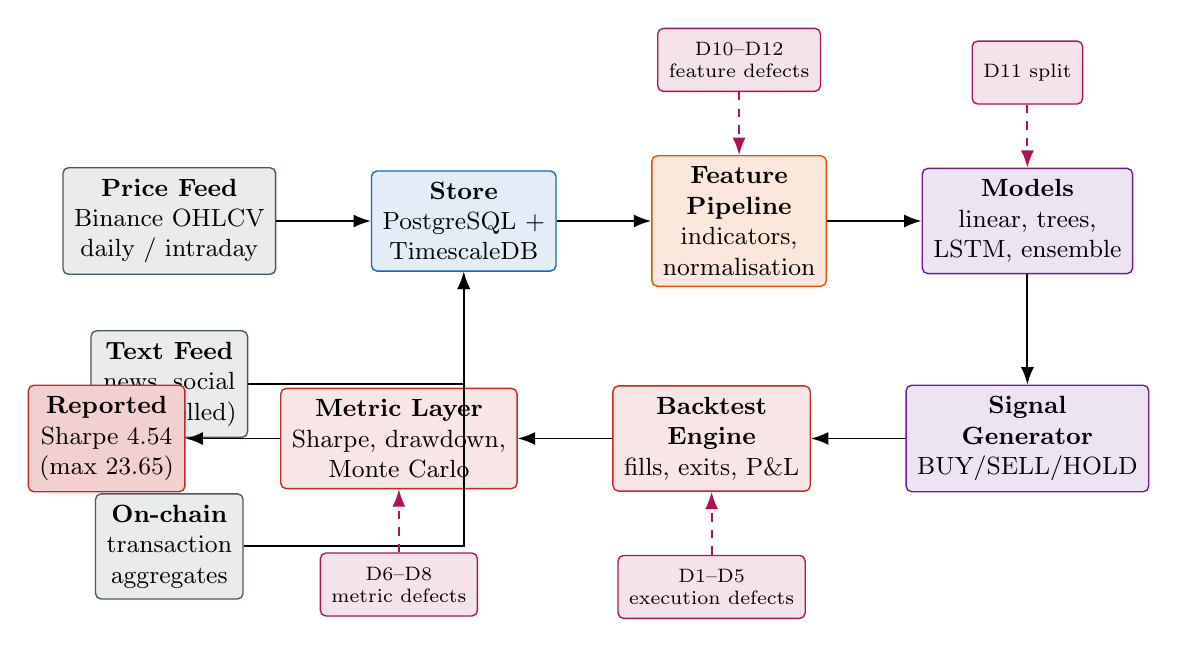
\begin{tikzpicture}[node distance=7mm and 12mm]
\node[io] (px)   {\textbf{Price Feed}\\ Binance OHLCV\\ daily / intraday};
\node[io, below=of px] (news) {\textbf{Text Feed}\\ news, social\\ (unlabelled)};
\node[io, below=of news] (chain) {\textbf{On-chain}\\ transaction\\ aggregates};
\node[dnode, right=of px] (store) {\textbf{Store}\\ PostgreSQL +\\ TimescaleDB};
\node[pnode, right=of store] (feat) {\textbf{Feature}\\ \textbf{Pipeline}\\ indicators,\\ normalisation};
\node[enode, right=of feat] (model) {\textbf{Models}\\ linear, trees,\\ LSTM, ensemble};
\node[enode, below=14mm of model] (sig) {\textbf{Signal}\\ \textbf{Generator}\\ BUY/SELL/HOLD};
\node[bnode, left=of sig] (bt) {\textbf{Backtest}\\ \textbf{Engine}\\ fills, exits, P\&L};
\node[bnode, left=of bt] (met) {\textbf{Metric Layer}\\ Sharpe, drawdown,\\ Monte Carlo};
\node[io, left=of met, fill=cBad!22, draw=cBad] (rep) {\textbf{Reported}\\ Sharpe $4.54$\\ (max $23.65$)};
\draw[arr] (px)--(store); \draw[arr] (news)-|(store); \draw[arr] (chain)-|(store);
\draw[arr] (store)--(feat); \draw[arr] (feat)--(model); \draw[arr] (model)--(sig);
\draw[arr] (sig)--(bt); \draw[arr] (bt)--(met); \draw[arr] (met)--(rep);
\node[wnode, above=8mm of feat, font=\scriptsize] (d1) {D10--D12\\ feature defects};
\node[wnode, above=8mm of model, font=\scriptsize] (d2) {D11 split};
\draw[darr, draw=cWarn] (d1)--(feat); \draw[darr, draw=cWarn] (d2)--(model);
\node[wnode, below=8mm of bt, font=\scriptsize] (d3) {D1--D5\\ execution defects};
\node[wnode, below=8mm of met, font=\scriptsize] (d4) {D6--D8\\ metric defects};
\draw[darr, draw=cWarn] (d3)--(bt); \draw[darr, draw=cWarn] (d4)--(met);
\end{tikzpicture}}
\caption{The pipeline under audit, with the twelve defects of
Section~\ref{sec:defects} located at the stage where each occurs. No defect lies
in the model families themselves.}
\label{fig:system}
\end{figure}

The audited system used a single backtest engine shared by an HTTP API and a batch
worker, a metric module of roughly 360 lines, and a feature pipeline that served
both training and inference. The evaluation it published covered ten
symbol/interval series with, in its own description, ``the latest 900 rows per
available symbol/interval''. We note in passing that $900$ fifteen-minute bars is
$9.4$ days; the same row count was applied uniformly across intervals, so the most
favourable-looking results in the published table were drawn from under two weeks
of data.

%==============================================================================
\section{A Taxonomy of Evaluation Defects}
\label{sec:defects}
%==============================================================================

We group the twelve defects into three families: execution defects, which corrupt
the simulated trade record; metric defects, which corrupt statistics computed from
a correct record; and pipeline defects, which corrupt the model input itself.
Table~\ref{tab:defects} summarises. Each is described below with its mechanism and
its correction.

\begin{table}[t]\centering\small
\caption{The twelve defects, their family, and the direction of their effect on
reported performance. Every defect is covered by at least one regression test in
the released harness.}
\label{tab:defects}
\begin{tabular}{@{}clll@{}}
\toprule
ID & Family & Defect & Effect \\
\midrule
D1  & Execution & Position priced from another asset & Corrupts \\
D2  & Execution & Nearest-bar lookup selects future bar & Inflates \\
D3  & Execution & Fill at signal bar close (no lag) & Inflates \\
D4  & Execution & Short mark-to-market sign inverted & Corrupts \\
D5  & Execution & Exits checked only at signal arrival, on close & Inflates \\
D6  & Metric    & Per-trade returns annualised by $\sqrt{252}$ & Inflates \\
D7  & Metric    & Monte Carlo permutation-invariant & Voids \\
D8  & Metric    & Calmar uses worst trade, not drawdown & Corrupts \\
D9  & Metric    & Accuracy relabelled as Sharpe / profit factor & Misleads \\
D10 & Pipeline  & Scaler fitted on one row at inference & Voids \\
D11 & Pipeline  & Train/test split without embargo & Inflates \\
D12 & Pipeline  & Imputation statistic computed over full sample & Inflates \\
\bottomrule
\end{tabular}
\end{table}

\subsection{Execution defects}

\paragraph{D1: cross-asset position pricing.}
The simulation loop iterated over signals. At each signal it resolved a price for
that signal asset, then passed the \emph{same} price into the exit check for every
open position regardless of asset. In a multi-asset run a Bitcoin position could
therefore be stopped out at Dogecoin price. Since the audited evaluation reported
BTC, ETH and DOGE jointly, every multi-asset trade in the published table was
affected. The correction is to iterate over bars rather than signals and price
each position from its own series.

\paragraph{D2: look-ahead in the price lookup.}
The price resolver selected the bar minimising $|t_{\text{bar}} - t_{\text{signal}}|$.
For any signal timestamp not exactly on a bar boundary this can select a bar that
has not yet occurred. The correction constrains the search to $t_{\text{bar}} \le
t_{\text{signal}}$ via binary search:
\begin{equation}
i^\star = \max \{\, i : t_i \le t_{\text{signal}} \,\}.
\end{equation}

\paragraph{D3: absent implementation lag.}
Signals derived from the close of bar $i$ were filled at the close of bar $i$. This
assumes an execution simultaneous with the information that generated it. We fill
at the open of bar $i+1$ instead. Section~\ref{ssec:e2e} shows this single change
is worth roughly $0.45$ of annualised Sharpe on our data, which is larger than the
entire gross signal.

\paragraph{D4: inverted short mark-to-market.}
Portfolio value was computed as $\sum_j q_j p_t^{(j)}$ over all open positions. For
a short position this rises as the price rises. The equity curve, and every
statistic derived from it, was therefore sign-inverted whenever a short was open.
The correction carries the short as a liability,
\begin{equation}
V_t = \text{cash}_t + \sum_{j \in \text{long}} q_j p_t^{(j)} - \sum_{j \in \text{short}} q_j p_t^{(j)}.
\label{eq:equity}
\end{equation}

\paragraph{D5: unsimulated stops.}
Stop and target conditions were evaluated only inside the signal loop, and only
against the bar close. A stop was therefore checked only when an unrelated signal
happened to arrive, and intrabar breaches were invisible. The correction evaluates
every open position against every bar, using the bar high and low:
\begin{equation}
\text{exit}=
\begin{cases}
\text{stop}   & \ell_t \le S \quad (\text{long}), \\
\text{target} & h_t \ge T \quad (\text{long, and stop not hit}), \\
\text{timeout}& t - t_{\text{entry}} \ge \tau.
\end{cases}
\end{equation}
When a single bar touches both levels the ordering is unidentifiable from OHLC, so
we resolve pessimistically to the stop.

\subsection{Metric defects}

\paragraph{D6: annualisation of per-trade returns.}
The Sharpe ratio was computed as $\bar{r}/\sigma_r \times \sqrt{252}$ where $r$ was
the vector of \emph{per-trade} returns. Trades do not arrive on a fixed clock, so
no single annualisation factor is defined for them. This is the single largest
contributor to the reported $23.65$. The correction computes returns from the
equity curve sampled at the bar cadence and derives the factor from the observed
spacing,
\begin{equation}
S = \frac{\overline{r - r_f}}{\sigma_{r - r_f}}\sqrt{P},
\qquad
P = \frac{\text{seconds per year}}{\mathrm{median}\,\{t_{i+1} - t_i\}}.
\label{eq:sharpe}
\end{equation}
A fifteen-minute series annualises by $\sqrt{35040}$ and a daily series by
$\sqrt{365}$; a second implementation elsewhere in the same codebase hardcoded the
former and applied it to a per-signal-event curve, so the two implementations
disagreed with each other as well as with the definition.

\paragraph{D7: a permutation-invariant Monte Carlo.}
The bootstrap routine shuffled the trade profit-and-loss vector and summed it:
\begin{equation}
\text{sim}_k = \sum_{i} \pi_k(x)_i = \sum_i x_i \quad \text{for every permutation } \pi_k.
\end{equation}
Summation is invariant under permutation, so all $1{,}000$ simulated paths returned
the identical value, the confidence interval collapsed to a point, and the reported
probability of profit was always exactly $0$ or $1$. The correction resamples with
replacement and tracks the order-dependent statistic that motivates the exercise:
\begin{equation}
\text{DD}_k = \max_{m} \left( \max_{j \le m} \sum_{i \le j} x^{(k)}_i - \sum_{i \le m} x^{(k)}_i \right).
\end{equation}

\paragraph{D8: Calmar denominator.}
The Calmar ratio divided cumulative return by $|\min_i r_i|$, the worst single
trade. Calmar is defined against peak-to-trough drawdown of the equity curve, which
the same module computed correctly elsewhere and did not use.

\paragraph{D9: accuracy in the costume of risk.}
The trainer reported fields named \texttt{sharpe\_ratio} and
\texttt{profit\_factor} constructed by assigning $+1$ to each correct prediction
and $-1$ to each incorrect one. For accuracy $a$ these are deterministic
transforms,
\begin{equation}
\text{``Sharpe''} = \frac{2a-1}{2\sqrt{a(1-a)}},
\qquad
\text{``profit factor''} = \frac{a}{1-a},
\end{equation}
carrying no information beyond $a$ itself while presenting as risk and
profitability measures. We replaced them with a Wald interval and a binomial test
(Section~\ref{ssec:stats}).

\subsection{Pipeline defects}

\paragraph{D10: the single-row scaler.}
At inference the feature vector was standardised by calling
\texttt{StandardScaler().fit\_transform(X)} on a single row. With one sample per
column the sample mean equals the observation and the variance is zero, so the
output is identically zero:
\begin{equation}
z = \frac{x - \mu}{\sigma} \bigg|_{\mu = x,\ \sigma \to 1} = 0.
\end{equation}
Every served prediction was therefore made on a zero vector. The scaler was also
re-instantiated per call, so no fitted statistics ever persisted from training. We
separate fitting from transformation, persist the fitted object with the model
artefacts, and warn rather than silently zero when no fitted scaler is loaded.

\paragraph{D11: split without embargo.}
Training samples were $60$-step windows whose labels referenced the following bar,
and some features used rolling windows up to $672$ bars. The split was a plain
$80/20$ index cut. Windows adjacent to the cut therefore shared underlying bars
across the boundary, so validation accuracy was measured partly on training data.
We introduce an embargo of at least the sequence length plus the label horizon,
\begin{equation}
\mathcal{T}_{\text{train}} = [0, k), \qquad
\mathcal{T}_{\text{test}} = [k + e, n), \qquad
e \ge L_{\text{seq}} + h .
\label{eq:embargo}
\end{equation}
This is the purge-and-embargo construction of \citet{lopezdeprado2018advances}.

\paragraph{D12: imputation over the full sample.}
Missing values were filled with the column mean computed over the entire frame,
including future rows. Forward-fill is causal; a global mean is not. We restrict
imputation to forward-fill and fit all remaining statistics inside the training
fold.

\subsection{A note on how these defects interact}

Individually several of these would be caught by inspection. What made them
survive is that they \emph{compensate}. D4 corrupts the equity curve, but D6
computed Sharpe from the trade record rather than the curve, so the corruption did
not surface in the headline number. D10 zeroed the served features, but the
reported accuracy came from a separate offline path that did not use the serving
code. The published metrics were each computed by a path that did not exercise the
defect most likely to have been noticed. This is, we suspect, the general case
rather than an unlucky one, and it is the argument for testing the instrument
directly rather than inspecting outputs for plausibility.

%==============================================================================
\section{Case Study: A Feature That Was the Label}
\label{sec:leakage}
%==============================================================================

The most consequential defect deserves separate treatment, because it would have
survived every correction in Section~\ref{sec:defects}.

\subsection{Mechanism}

The pipeline consumed a per-asset daily sentiment series with fields
\texttt{sentiment\_score}, \texttt{sentiment\_label} and
\texttt{simulated\_headline}. Tracing its provenance, the series is generated from
the price data itself:
\begin{align}
r^{\text{same}}_t &= \frac{C_t - O_t}{O_t}, \\
s_t &= \mathrm{clip}\!\left(15\, r^{\text{same}}_t,\, -1,\, 1\right) + \epsilon_t,
\qquad \epsilon_t \sim \mathcal{U}(-0.2, 0.2),
\label{eq:sentgen}
\end{align}
with the headline text drawn from fifteen fixed templates selected by the sign and
magnitude of $s_t$. The feature named sentiment is a clipped, noised, rescaled copy
of the same day open-to-close return. Figure~\ref{fig:leak} shows the construction.

\begin{figure}[t]\centering
\resizebox{0.95\textwidth}{!}{%
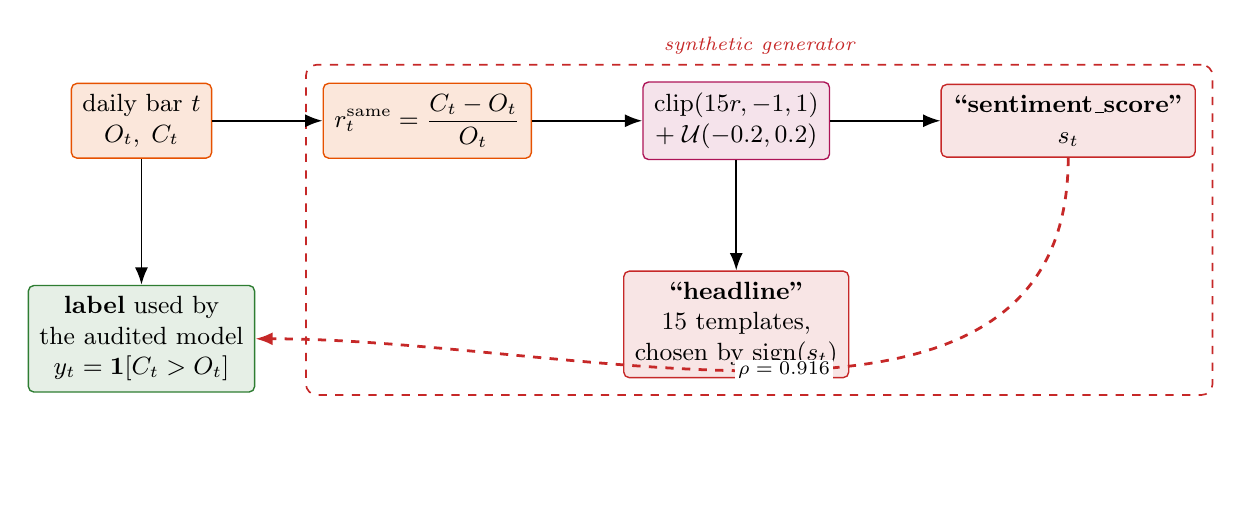
\begin{tikzpicture}[node distance=8mm and 14mm]
\node[pnode] (ohlc) {daily bar $t$\\ $O_t,\;C_t$};
\node[pnode, right=of ohlc] (ret) {$r^{\text{same}}_t=\dfrac{C_t-O_t}{O_t}$};
\node[wnode, right=of ret] (scale) {$\mathrm{clip}(15r,-1,1)$\\ $+\;\mathcal{U}(-0.2,0.2)$};
\node[bnode, right=of scale] (sent) {\textbf{``sentiment\_score''}\\ $s_t$};
\node[bnode, below=14mm of scale] (head) {\textbf{``headline''}\\ 15 templates,\\ chosen by $\mathrm{sign}(s_t)$};
\node[gnode, below=16mm of ohlc] (lab) {\textbf{label} used by\\ the audited model\\ $y_t=\mathbf{1}[C_t>O_t]$};
\draw[arr] (ohlc)--(ret); \draw[arr] (ret)--(scale); \draw[arr] (scale)--(sent);
\draw[arr] (scale)--(head);
\draw[arr] (ohlc)--(lab);
\draw[darr, draw=cBad, line width=1pt] (sent.south) to[out=-90,in=0]
      node[lbl,pos=0.5]{$\rho=0.916$} (lab.east);
\begin{scope}[on background layer]
  \node[group, draw=cBad, fit=(ret)(scale)(sent)(head), label={[font=\scriptsize\itshape,text=cBad]above:synthetic generator}] {};
\end{scope}
\end{tikzpicture}}
\caption{The leakage mechanism. The feature marketed as sentiment is generated
from the same bar that generates the label, so the two share a common
deterministic parent. No text is involved at any point.}
\label{fig:leak}
\end{figure}

\subsection{Quantification}

Table~\ref{tab:leak} measures the resulting dependence on BTC daily bars over the
full sample.

\begin{table}[t]\centering\small
\caption{Dependence between the sentiment-named feature and returns, BTC daily,
$n = 3{,}150$. The feature is strongly informative about the contemporaneous
return and uninformative about the future.}
\label{tab:leak}
\begin{tabular}{@{}lrr@{}}
\toprule
Relationship & Pearson $\rho$ & Sign agreement \\
\midrule
\texttt{sentiment\_score} vs.\ \textbf{same-day} return  & $0.916$  & $87.0\%$ \\
\texttt{sentiment\_score} vs.\ \textbf{next-day}  return & $-0.018$ & $47.2\%$ \\
\bottomrule
\end{tabular}
\end{table}

Two consequences follow. First, any model using $s_t$ to predict the sign of
$r^{\text{same}}_t$ has near-direct access to its own label and will report
accuracy in the high eighties. Second, and less obviously, using $s_t$ to predict
$r_{t+1}$ is \emph{not} leakage in the formal sense -- $s_t$ is known at the close
of day $t$ -- but it is also worthless, contributing nothing beyond a momentum
term while carrying a name that implies an independent information source.

\subsection{Why this class of defect is hard to catch}

Standard leakage detection looks for features whose distribution shifts across the
train/test boundary, or for suspiciously high validation scores. Neither fires
here. The generator adds enough noise that the mapping is not exactly invertible,
so the accuracy it produces is high but not perfect. The feature has a plausible
name, a plausible range, an accompanying text field, and a documented ingestion
script. The failure is one of \emph{provenance}, not of statistics, and provenance
is not visible in the feature matrix.

We therefore recommend that any feature claimed to derive from an exogenous source
be accompanied by a provenance test: an assertion, in the test suite, that the
feature cannot be reconstructed from contemporaneous market data above some
threshold $R^2$. We include such a test in the released harness.

We exclude the sentiment series entirely from all results that follow. The dataset
contains no genuine timestamped sentiment labels, and consequently this paper
makes no claim regarding sentiment-driven prediction.

%==============================================================================
\section{Methodology}
\label{sec:method}
%==============================================================================

\subsection{Data}

We use Binance daily OHLCV for BTCUSDT, ETHUSDT and DOGEUSDT. The raw series run
from the Binance listing of each asset to 2026-03-31. After a $60$-day warm-up
required by the longest rolling feature, the usable ranges are those in
Table~\ref{tab:data}. Beyond the standard OHLCV fields we retain three columns
from the Binance kline payload that carry genuine microstructure information:
number of trades, quote asset volume, and taker buy base asset volume.

\begin{table}[t]\centering\small
\caption{Evaluated data coverage after feature warm-up.}
\label{tab:data}
\begin{tabular}{@{}lrrrr@{}}
\toprule
Asset & Usable bars & Start & End & Folds \\
\midrule
BTCUSDT  & $3{,}089$ & 2017-10-16 & 2026-03-31 & 9 \\
ETHUSDT  & $3{,}089$ & 2017-10-16 & 2026-03-31 & 9 \\
DOGEUSDT & $2{,}402$ & 2019-09-03 & 2026-03-31 & 6 \\
\bottomrule
\end{tabular}
\end{table}

\subsection{Features}

We compute $34$ features, all strictly causal in the sense that each is a function
of bars indexed $\le t$. They fall into five groups:

\begin{itemize}
\item \textbf{Returns.} Log returns over horizons $\{1,2,3,5,10,20\}$ days.
\item \textbf{Volatility and location.} Rolling standard deviation of log returns
and a rolling $z$-score of close, each over $\{5,10,20,60\}$ days.
\item \textbf{Bar shape.} High-low range normalised by close, close-open spread
normalised by open, and the location of the close within the bar range.
\item \textbf{Order flow.} Taker buy ratio and its five-day mean, average trade
size and its $60$-day $z$-score, $z$-scored trade count, $z$-scored volume, and
volume relative to its $20$-day mean. These derive from real exchange fields and
are the only genuinely non-price information in the study.
\item \textbf{Technical indicators.} RSI(14), MACD histogram (12/26/9), Bollinger
position, ATR(14) normalised by close, and a sine/cosine encoding of day of week.
\end{itemize}

Full definitions appear in \ref{app:features}.

\subsection{Labels}

The primary label is the sign of the next daily close-to-close return,
\begin{equation}
y_t = \mathbf{1}\!\left[\, C_{t+1} > C_t \,\right],
\qquad
r_{t+1} = \frac{C_{t+1}}{C_t} - 1 .
\end{equation}
We deliberately do not use a neutral dead-band. A three-class formulation with an
abstention region reports a more flattering accuracy, but it changes the null
hypothesis in a way that is easy to misreport and it complicates the mapping to a
tradable position. The binary formulation admits an unambiguous $50\%$ null.

\subsection{Validation protocol}

We use expanding-window walk-forward validation with an embargo
(Figure~\ref{fig:wf}). The first test fold begins after $1{,}000$ training days;
each fold tests $250$ days; the training set expands to include all data preceding
the embargo. The embargo is $5$ days, exceeding the one-day label horizon with
margin.

\begin{figure}[t]\centering
\resizebox{0.95\textwidth}{!}{%
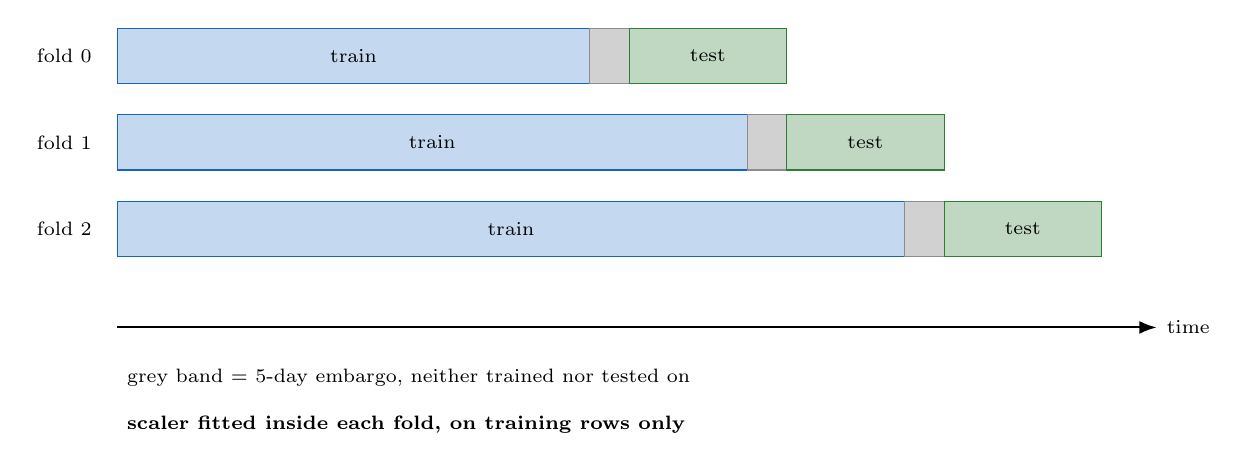
\begin{tikzpicture}[x=1mm,y=1mm]
\foreach \k/\tr in {0/60, 1/80, 2/100}{
  \pgfmathsetmacro{\yy}{-\k*11}
  \pgfmathsetmacro{\eb}{\tr+5}
  \pgfmathsetmacro{\tb}{\tr+25}
  \node[font=\scriptsize,anchor=east] at (-2,\yy+3.5) {fold \k};
  \draw[fill=cData!25,draw=cData] (0,\yy) rectangle (\tr,\yy+7);
  \node[font=\scriptsize] at (\tr/2,\yy+3.5) {train};
  \draw[fill=black!18,draw=black!45] (\tr,\yy) rectangle (\eb,\yy+7);
  \draw[fill=cGood!30,draw=cGood] (\eb,\yy) rectangle (\tb,\yy+7);
  \node[font=\scriptsize] at (\eb+10,\yy+3.5) {test};
}
\draw[arr] (0,-31) -- (132,-31) node[right,font=\scriptsize] {time};
\node[font=\scriptsize,anchor=north west] at (0,-35)
  {grey band = 5-day embargo, neither trained nor tested on};
\node[font=\scriptsize,anchor=north west] at (0,-41)
  {\textbf{scaler fitted inside each fold, on training rows only}};
\end{tikzpicture}}
\caption{Expanding-window walk-forward with embargo. The embargo interval is
discarded, never trained or tested on, so no bar contributes to both sides of a
split.}
\label{fig:wf}
\end{figure}

Critically, the feature scaler is fitted \emph{inside each fold} on training rows
only, and applied unchanged to the test rows. Fitting a scaler on the full sample
leaks the test period mean and variance into the training representation; this is
a small effect relative to the defects of Section~\ref{sec:defects} but it is free
to avoid.

\subsection{Models}

\begin{itemize}
\item \textbf{Logistic}: $\ell_2$-regularised logistic regression, $C = 0.1$.
\item \textbf{GBDT}: histogram gradient-boosted trees, depth $3$, $200$ iterations,
learning rate $0.05$, $\ell_2$ regularisation $1.0$.
\end{itemize}

Hyperparameters were fixed a priori at conventional values and not tuned on test
data. We report both models in full rather than selecting one.

\subsection{Baselines}

Three baselines are computed over identical windows.
\begin{itemize}
\item \textbf{Persistence}: $\hat{y}_t = y_{t-1}$, the naive forecast that today
direction repeats.
\item \textbf{Majority}: the more frequent class in the training fold, held fixed
across the test window.
\item \textbf{Buy-and-hold}: passive long exposure, reported as annualised Sharpe.
\end{itemize}

\subsection{Statistical reporting}
\label{ssec:stats}

For a hit rate $a$ over $n$ independent predictions we report the Wald interval
and a two-sided test against the coin-flip null,
\begin{equation}
a \pm 1.96\sqrt{\frac{a(1-a)}{n}},
\qquad
z = \frac{a - 0.5}{\sqrt{0.25/n}},
\qquad
p = \mathrm{erfc}\!\left(\frac{|z|}{\sqrt{2}}\right).
\label{eq:stats}
\end{equation}
We report $n$ alongside every accuracy. An accuracy without $n$ and without a
baseline is not interpretable, and the absence of these was among the defects we
catalogued.

\subsection{Execution and cost model}

The corrected engine implements the timing of Figure~\ref{fig:timing}: a signal
computed from the close of day $t$ is filled at the open of day $t+1$ and exits at
the close of day $t+2$ under a $24$-hour timeout, or earlier at a barrier. Costs
are $4$ bps taker fee plus $5$ bps slippage, charged per side on the notional of
that leg.

\begin{figure}[t]\centering
\resizebox{0.9\textwidth}{!}{%
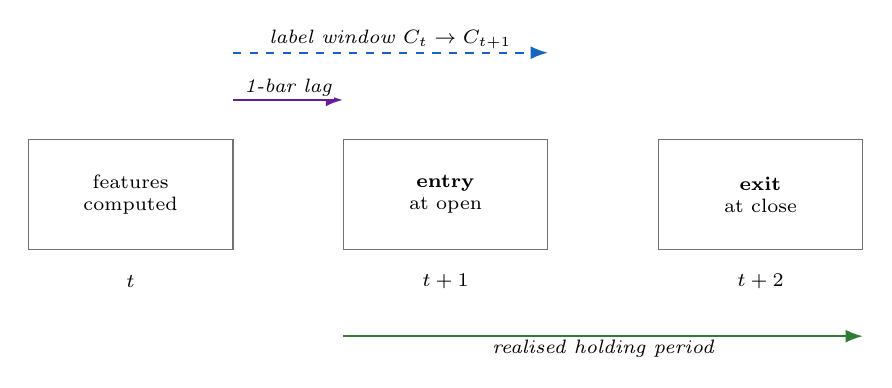
\begin{tikzpicture}[x=1mm,y=1mm]
\draw[draw=black!55] (0,0)  rectangle (26,14);
\draw[draw=black!55] (40,0) rectangle (66,14);
\draw[draw=black!55] (80,0) rectangle (106,14);
\node[font=\scriptsize] at (13,-4) {$t$};
\node[font=\scriptsize] at (53,-4) {$t+1$};
\node[font=\scriptsize] at (93,-4) {$t+2$};
\node[font=\scriptsize,align=center] at (13,7)  {features\\ computed};
\node[font=\scriptsize,align=center] at (53,7)  {\textbf{entry}\\ at open};
\node[font=\scriptsize,align=center] at (93,7)  {\textbf{exit}\\ at close};
\draw[arr,draw=cEval,line width=1pt] (26,19) -- node[lbl,above]{1-bar lag} (40,19);
\draw[arr,draw=cGood] (40,-11) -- node[lbl,below]{realised holding period} (106,-11);
\draw[arr,draw=cData,dashed] (26,25) -- node[lbl,above]{label window $C_t \to C_{t+1}$} (66,25);
\end{tikzpicture}}
\caption{Execution timing in the corrected engine. The label window and the
realised holding period do not coincide; the gap between them is quantified in
Section~\ref{ssec:e2e}.}
\label{fig:timing}
\end{figure}

%==============================================================================
\section{Results}
\label{sec:results}
%==============================================================================

\subsection{Directional accuracy}
\label{ssec:accuracy}

Table~\ref{tab:acc} reports out-of-sample accuracy per asset and pooled.

\begin{table}[t]\centering\small
\caption{Walk-forward out-of-sample directional accuracy. Gross Sharpe is the
annualised Sharpe of acting on every signal with no transaction costs. Baseline
rows are computed over identical windows.}
\label{tab:acc}
\begin{tabular}{@{}llrrcrr@{}}
\toprule
Asset & Model & $n$ & Accuracy & 95\% CI & $p$ & Gross SR \\
\midrule
\multirow{4}{*}{BTC}
 & Logistic     & $2{,}084$ & $52.74\%$ & $[50.59, 54.88]$ & $0.013$ & $0.44$ \\
 & GBDT         & $2{,}084$ & $52.11\%$ & $[49.97, 54.26]$ & $0.054$ & $-0.01$ \\
 & Persistence  & $2{,}084$ & $46.98\%$ & --- & $0.006$ & --- \\
 & Majority     & $2{,}084$ & $50.53\%$ & --- & $0.630$ & --- \\
\midrule
\multirow{4}{*}{ETH}
 & Logistic     & $2{,}084$ & $53.07\%$ & $[50.93, 55.21]$ & $0.005$ & $0.41$ \\
 & GBDT         & $2{,}084$ & $51.34\%$ & $[49.20, 53.49]$ & $0.220$ & $0.36$ \\
 & Persistence  & $2{,}084$ & $47.46\%$ & --- & $0.020$ & --- \\
 & Majority     & $2{,}084$ & $49.62\%$ & --- & $0.726$ & --- \\
\midrule
\multirow{4}{*}{DOGE}
 & Logistic     & $1{,}397$ & $53.04\%$ & $[50.43, 55.66]$ & $0.023$ & $0.61$ \\
 & GBDT         & $1{,}397$ & $51.90\%$ & $[49.28, 54.52]$ & $0.156$ & $0.39$ \\
 & Persistence  & $1{,}397$ & $46.89\%$ & --- & $0.020$ & --- \\
 & Majority     & $1{,}397$ & $51.68\%$ & --- & $0.209$ & --- \\
\midrule
\multirow{2}{*}{\textbf{Pooled}}
 & \textbf{Logistic} & $\mathbf{5{,}565}$ & $\mathbf{52.94\%}$ & $\mathbf{[51.63, 54.25]}$ & $\mathbf{<10^{-4}}$ & $\mathbf{0.60}$ \\
 & GBDT              & $5{,}565$ & $51.77\%$ & $[50.46, 53.08]$ & $0.008$ & --- \\
\bottomrule
\end{tabular}
\end{table}

Three observations.

First, the pooled logistic result is unambiguous on its own terms: $z = 4.38$,
$p < 10^{-4}$. It is not a marginal finding, and it survives the Bonferroni
correction for the two models tried by a wide margin.

Second, the regularised linear model beats the gradient-boosted ensemble on every
asset. GBDT reaches conventional significance only in the pooled sample. This is
the expected ordering in a low signal-to-noise regime, where flexible models spend
capacity fitting noise, and is consistent with \citet{gu2020empirical}.

Third, persistence performs at $47\%$, significantly \emph{worse} than chance. This
is itself informative: daily crypto returns exhibit mild short-horizon reversal, so
a naive momentum forecast is systematically wrong. Part of what the models learn is
to invert this tendency, and a study reporting only accuracy against a $50\%$ null
without the persistence baseline would overstate how much has been learned.

\subsection{Cost sensitivity and breakeven}
\label{ssec:costs}

Statistical significance says nothing about tradability. We construct an
equal-weight daily long/short book from the logistic signal, with position
$\pi_t \in \{-1, +1\}$ per asset, and charge turnover at a variable rate,
\begin{equation}
r^{\text{net}}_t = \pi_t r_{t+1} - c\,\lvert \pi_t - \pi_{t-1} \rvert .
\end{equation}
Average daily turnover is $0.774$. Figure~\ref{fig:cost} and Table~\ref{tab:cost}
show annualised Sharpe as a function of $c$.

\begin{figure}[t]\centering
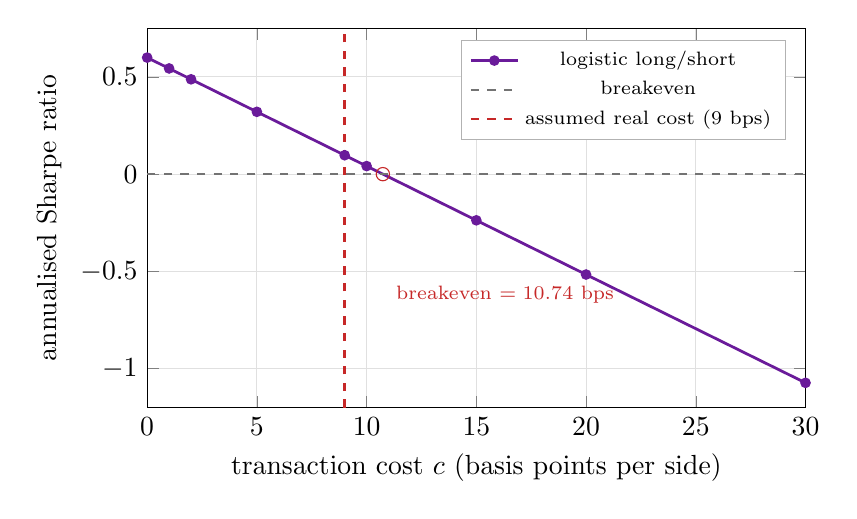
\begin{tikzpicture}
\begin{axis}[width=0.82\textwidth,height=6.4cm,
    xlabel={transaction cost $c$ (basis points per side)},
    ylabel={annualised Sharpe ratio},
    xmin=0,xmax=30,ymin=-1.2,ymax=0.75,
    grid=major,grid style={black!12},
    legend pos=north east,legend style={font=\scriptsize,draw=black!30}]
\addplot[color=cEval,mark=*,mark size=1.4pt,line width=1pt] coordinates {
  (0,0.599) (1,0.5433) (2,0.4875) (5,0.3203) (9,0.0972)
  (10,0.0415) (15,-0.2373) (20,-0.516) (30,-1.0726)};
\addlegendentry{logistic long/short}
\addplot[color=black!55,dashed,line width=0.7pt] coordinates {(0,0)(30,0)};
\addlegendentry{breakeven}
\addplot[color=cBad,dashed,line width=0.9pt] coordinates {(9,-1.2)(9,0.75)};
\addlegendentry{assumed real cost (9 bps)}
\node[font=\scriptsize,anchor=west,text=cBad] at (axis cs:10.9,-0.62)
     {breakeven $=10.74$ bps};
\addplot[color=cBad,only marks,mark=o,mark size=2.4pt] coordinates {(10.74,0)};
\end{axis}
\end{tikzpicture}
\caption{Annualised Sharpe of the logistic long/short book against transaction
cost. The strategy crosses zero at $10.74$ bps per side; realistic costs are
approximately $9$ bps.}
\label{fig:cost}
\end{figure}

\begin{table}[t]\centering\small
\caption{Cost sensitivity of the logistic long/short book, $1{,}397$ overlapping
trading days.}
\label{tab:cost}
\begin{tabular}{@{}lrrrrrrr@{}}
\toprule
Cost (bps/side) & $0$ & $2$ & $5$ & $\mathbf{9}$ & $10$ & $15$ & $20$ \\
\midrule
Annualised Sharpe & $0.60$ & $0.49$ & $0.32$ & $\mathbf{0.10}$ & $0.04$ & $-0.24$ & $-0.52$ \\
\bottomrule
\end{tabular}
\end{table}

The breakeven cost is $10.74$ bps per side. Against an assumed $9$ bps the
strategy retains an annualised Sharpe of $0.10$, which is statistically
indistinguishable from zero over this sample. We regard the breakeven figure as
the more informative statistic than any single net Sharpe, because it is invariant
to the analyst choice of cost assumption -- precisely the choice most available for
motivated reasoning.

\subsection{End-to-end simulation}
\label{ssec:e2e}

Table~\ref{tab:bt} reports the same signals run through the corrected engine, which
adds the one-bar implementation lag of Figure~\ref{fig:timing}, discrete position
sizing, and a one-position-per-asset constraint.

\begin{table}[t]\centering\small
\caption{End-to-end backtest, logistic signals through the corrected engine,
2017-08-17 to 2026-04-01.}
\label{tab:bt}
\begin{tabular}{@{}lr@{}}
\toprule
Metric & Value \\
\midrule
Trades                    & $5{,}562$ \\
Win rate                  & $50.02\%$ \\
Mean return per trade     & $-0.094\%$ \\
Total return              & $-70.45\%$ \\
Maximum drawdown          & $72.73\%$ \\
Profit factor             & $0.920$ \\
\textbf{Annualised Sharpe}& $\mathbf{-0.346}$ \\
\bottomrule
\end{tabular}
\end{table}

The gap between $+0.10$ under the frictionless-timing cost model and $-0.346$ under
realistic execution is, we argue, the most practically important number in the
paper. It is not a discrepancy between two estimates of the same quantity; it is a
measurement of how much of the edge is consumed by acting one bar late. The signal
predicts the close-to-close window $C_t \to C_{t+1}$, and an implementation that
cannot enter until the open of $t+1$ has already forfeited the overnight gap, which
in crypto markets carries a disproportionate share of the move.

A study that reports the label-window Sharpe and describes it as strategy
performance is not making an arithmetic error, but it is reporting a quantity no
participant can realise.

\subsection{Before and after}

Table~\ref{tab:beforeafter} places the corrected results beside the originals.

\begin{table}[t]\centering\small
\caption{Reported performance before and after the corrections of
Section~\ref{sec:defects}. The original figures are those published by the audited
system; the corrected figures are from this study.}
\label{tab:beforeafter}
\begin{tabular}{@{}lrr@{}}
\toprule
Quantity & Original & Corrected \\
\midrule
Aggregate annualised Sharpe   & $4.54$   & $-0.35$ \\
Maximum per-series Sharpe     & $23.65$  & --- \\
Directional accuracy          & $52.44\%$& $52.94\%$ \\
Reported with CI and $p$      & no       & yes \\
Win rate                      & $30.23\%$& $50.02\%$ \\
Trades                        & $210$    & $5{,}562$ \\
Evaluation window (15m series)& $9.4$ days & $8.6$ years (daily) \\
Baselines reported            & none     & three \\
\bottomrule
\end{tabular}
\end{table}

The directional accuracy is the one quantity that survives essentially unchanged.
This is not a coincidence: accuracy was computed on an offline path that did not
exercise the execution or metric defects. Everything downstream of it moved by
more than its own magnitude.

%==============================================================================
\section{Verification: A Null-Test Protocol}
\label{sec:nulltest}
%==============================================================================

Correcting twelve defects raises an obvious question: how would we know if a
thirteenth remained? Inspecting outputs for plausibility is what failed in the
first place. We therefore propose testing the instrument against data whose correct
answer is known by construction.

\subsection{Construction}

Generate a driftless geometric random walk,
\begin{equation}
P_{t+1} = P_t \exp(\sigma \varepsilon_t), \qquad \varepsilon_t \sim \mathcal{N}(0,1),
\end{equation}
and emit entry signals with random side at random times. There is no predictable
structure, so a correct engine charging any positive cost must report
\begin{equation}
S \le 0 .
\label{eq:nullcond}
\end{equation}
We additionally require exact reconciliation between the trade record and the
equity curve. With all positions closed at the end,
\begin{equation}
V_T - V_0 = \sum_{i=1}^{N} \text{PnL}_i ,
\label{eq:reconcile}
\end{equation}
and separately that expectancy implied by the realised win rate and average
win/loss equal realised mean return per trade,
\begin{equation}
w\,\bar{g} + (1-w)\,\bar{\ell} \;=\; \frac{1}{N}\sum_i r_i .
\label{eq:expectancy}
\end{equation}

Equation~\eqref{eq:reconcile} is the strongest of the three. It is violated by any
defect that creates or destroys cash -- D1, D3, D4 and asymmetric fee charging all
fail it -- and it cannot be satisfied by accident.

\subsection{Result}

Table~\ref{tab:null} reports the protocol on $7{,}200$ synthetic bars per asset
across three assets.

\begin{table}[t]\centering\small
\caption{Null-test output on random signals over a driftless random walk. The
pre-correction engine reported positive Sharpe on this fixture; the corrected
engine reports the required non-positive value and reconciles exactly.}
\label{tab:null}
\begin{tabular}{@{}lrl@{}}
\toprule
Quantity & Value & Requirement \\
\midrule
Inferred periods per year & $35{,}040$ & $=\sqrt{}$-factor for 15m bars \\
Annualised Sharpe         & $-2.579$   & $\le 0$ \\
Profit factor             & $0.880$    & $< 1$ \\
Monte Carlo 95\% CI width & $1{,}720.4$& $> 0$ (non-degenerate) \\
Implied expectancy/trade  & $-0.1263\%$& \multirow{2}{*}{$\Big\}$ must be equal} \\
Realised expectancy/trade & $-0.1263\%$& \\
\bottomrule
\end{tabular}
\end{table}

The two expectancy figures agree to floating-point precision. The pre-correction
engine violated both \eqref{eq:nullcond} and \eqref{eq:expectancy} on this fixture.

\subsection{Proposal}

We suggest that a backtested performance claim be accompanied by the output of a
null test of this form, and that the reconciliation identity \eqref{eq:reconcile}
be stated as satisfied. Both are cheap -- the harness runs in under two seconds --
and neither requires disclosing the strategy. A null test does not establish that a
positive result is real, but it excludes a large and empirically common class of
ways for it to be spurious.

The released harness comprises $26$ regression tests: $17$ covering the execution
and metric defects, and $9$ covering the feature pipeline, including an assertion
that a single-row standardisation does not collapse to zero and that no bar appears
in both sides of a split.

%==============================================================================
\section{Discussion}
\label{sec:discussion}
%==============================================================================

\subsection{Statistical significance is not economic significance}

The central tension in our results is that a finding significant at $p < 10^{-4}$
is not tradable. This is not a paradox. With $n = 5{,}565$, the standard error on a
hit rate is $0.67$ percentage points, so an effect of $2.94$ points is easily
detected. But the economic value of a hit rate depends on the magnitude of the moves
captured, not on the confidence with which the rate differs from a half, and a
strategy trading daily at $77\%$ turnover pays roughly $14$ bps per day in costs at
$9$ bps per side.

The relationship is worth stating explicitly. For a symmetric long/short book the
gross Sharpe scales approximately as
\begin{equation}
S_{\text{gross}} \;\approx\; (2a-1)\,\frac{\sqrt{P}}{\text{IR-adjustment}},
\end{equation}
so accuracy enters linearly through $2a-1$, which at $a = 0.5294$ is $0.0588$.
Costs, in contrast, enter as a fixed subtraction proportional to turnover. There is
consequently a hit rate below which no amount of statistical confidence produces a
tradable strategy, and at daily frequency with these costs that threshold sits just
above where we are.

\subsection{Relation to market efficiency}

Our result matches the operational form of efficiency described by
\citet{timmermann2004efficient} more closely than either the strong or the naive
reading of \citet{fama1970efficient}. Predictability exists and is measurable. It
is small. It sits close enough to the cost boundary that it is plausibly the
residual left after arbitrage has removed whatever was profitable. That the
breakeven cost ($10.74$ bps) lands within striking distance of retail execution
cost ($9$ bps) is the kind of coincidence one should expect if costs are what
bounds the surviving inefficiency.

\subsection{Implications for practice}

Three recommendations follow from the audit.

\begin{enumerate}
\item \textbf{Test the instrument before the hypothesis.} Every defect we found
would have been caught by a fixture with a known answer, and none were caught by
years of plausibility inspection of outputs.
\item \textbf{Report breakeven cost, not net Sharpe.} A net Sharpe encodes an
assumption the reader cannot audit. A breakeven cost lets the reader supply their
own.
\item \textbf{Require provenance tests for exogenous features.} Any feature
claimed to carry information from outside the price series should be shown unable
to be reconstructed from contemporaneous market data.
\end{enumerate}

\subsection{On publishing the correction}

We report the original figures rather than quietly replacing them. This is
deliberate. The magnitude of the correction -- from $+4.54$ to $-0.35$ -- is itself
the evidence for the paper claim, and a reader cannot assess the argument without
it.

%==============================================================================
\section{Limitations and Threats to Validity}
\label{sec:limitations}
%==============================================================================

\paragraph{Model selection after seeing test results.}
We report both models we ran, but our narrative emphasises the logistic model,
chosen after observing out-of-sample results. With two candidates the multiplicity
cost is small, and GBDT is independently significant in the pooled sample
($p = 0.008$), so the qualitative conclusion is unaffected. A fully rigorous
treatment would apply the Deflated Sharpe Ratio of \citet{bailey2014deflated}; with
two trials the deflation is minor, but we note the exposure rather than assert its
irrelevance.

\paragraph{Overlapping observations.}
Pooling $5{,}565$ predictions across three assets treats them as independent. BTC
and ETH daily returns are strongly correlated, so the effective sample size is
smaller than the nominal one and the pooled $p$-value is optimistic. The per-asset
results, which do not pool, remain significant individually at conventional levels
for the logistic model, which is the more conservative reading.

\paragraph{Single frequency, three assets.}
We evaluate daily bars on three liquid cryptocurrencies. Nothing here establishes
what happens at hourly or minute frequency, where the cost calculus differs
substantially, nor on illiquid assets, where our cost assumption would be far too
generous.

\paragraph{Simplified cost model.}
We charge a flat per-side rate. Real execution involves a spread that widens with
volatility, market impact scaling with participation, and funding costs on short
positions. Our $9$ bps assumption is reasonable for retail taker execution in size
but is not a full transaction cost model, and the breakeven analysis should be read
as an approximation.

\paragraph{Survivorship and regime.}
The three assets were selected because data was available, and all three survived
to the end of the sample. The period spans two full crypto cycles, which is
favourable for generalisation, but a single asset class over eight years remains a
narrow base.

\paragraph{Absence of genuine sentiment data.}
The audited pipeline was built around a sentiment thesis we could not test, because
its sentiment data was synthetic. Whether real financial text adds forward
information over the feature set used here is an open question that this study does
not address.

%==============================================================================
\section{Conclusion}
\label{sec:conclusion}
%==============================================================================

We audited the evaluation stack of a working cryptocurrency trading system that
reported an annualised Sharpe ratio of $4.54$, isolated twelve defects spanning
execution, metric computation and the feature pipeline, and showed that the
reported figure was an artefact of the measurement apparatus rather than of any
predictive signal. Among the defects, the most instructive was a feature named for
sentiment that was in fact a scaled copy of the contemporaneous label,
correlating $0.916$ with the same day return and $-0.018$ with the next day.

Re-running the study under a corrected harness and a walk-forward protocol with
purge and embargo, we find weak but statistically robust directional structure:
$52.94\%$ accuracy over $5{,}565$ out-of-sample daily predictions,
$p < 10^{-4}$, against persistence at $47.0\%$ and majority at $50.5\%$. The same
signal has a gross annualised Sharpe of $0.60$, breaks even at $10.74$ basis points
per side against realistic costs near $9$, achieves $-0.346$ under realistic
execution timing, and does not beat buy-and-hold at $0.89$.

Both halves of that result matter. The field does not lack for reported edges; it
lacks reported edges that were measured on a calibrated instrument. We release the
harness, the null-test protocol and the $26$ regression tests in the hope that
verifying the instrument becomes an ordinary precondition for reporting a backtest
rather than an unusual one.

%==============================================================================
\section*{Data and code availability}
%==============================================================================

The evaluation harness, the corrected backtest engine, the null-test protocol and
all $26$ regression tests are released with this paper. The evaluation is
reproducible end to end from the released daily OHLCV data with a single command;
full numerical output is serialised to a machine-readable results file. No
proprietary data is used.

%==============================================================================
\appendix
%==============================================================================

\section{Feature definitions}
\label{app:features}

All features are functions of bars indexed $\le t$. Let $O_t, H_t, L_t, C_t, V_t$
denote the open, high, low, close and base volume, $Q_t$ the quote asset volume,
$N_t$ the trade count and $B_t$ the taker buy base volume.

\paragraph{Returns.} $\text{logret}_k(t) = \log(C_t / C_{t-k})$ for
$k \in \{1,2,3,5,10,20\}$.

\paragraph{Volatility and location.} For $k \in \{5,10,20,60\}$,
\[
\text{vol}_k(t) = \mathrm{sd}\big(\{\text{logret}_1(s)\}_{s=t-k+1}^{t}\big),
\qquad
\text{zclose}_k(t) = \frac{C_t - \mu_k(C)}{\sigma_k(C)} .
\]

\paragraph{Bar shape.}
\[
\text{hl\_range} = \frac{H_t - L_t}{C_t}, \quad
\text{co\_spread} = \frac{C_t - O_t}{O_t}, \quad
\text{close\_loc} = \frac{C_t - L_t}{H_t - L_t} .
\]

\paragraph{Order flow.}
\[
\text{taker\_buy\_ratio} = \frac{B_t}{V_t}, \qquad
\text{avg\_trade\_size} = \frac{Q_t}{N_t},
\]
each accompanied by a rolling mean or $60$-day $z$-score as described in
Section~\ref{sec:method}, together with $z$-scored $N_t$ and $V_t$ and the ratio
of $V_t$ to its $20$-day mean.

\paragraph{Technical indicators.}
RSI(14) from the ratio of mean gain to mean loss; MACD histogram as
$\text{EMA}_{12} - \text{EMA}_{26}$ minus its own $9$-period EMA; Bollinger
position $(C_t - \text{MA}_{20}) / (2\sigma_{20})$; ATR(14) as the $14$-day mean of
true range divided by $C_t$; and $\sin(2\pi d/7), \cos(2\pi d/7)$ for day of week
$d$.

\section{Corrected execution model}
\label{app:execution}

Let $\mathcal{B}^{(j)}$ be the ordered bar sequence for asset $j$. The engine
iterates over the union of timestamps. At each timestamp, for each asset with a bar
present, it first resolves exits for any open position in \emph{that} asset using
\emph{that} bar, then opens positions scheduled for that bar.

A signal timestamped within bar $i$ is scheduled for execution at bar $i+1$ and
filled at its open, adjusted by slippage $\varsigma$:
\begin{equation}
p_{\text{entry}} = O_{i+1}\,(1 + \varsigma) \text{ (long)}, \qquad
O_{i+1}\,(1 - \varsigma) \text{ (short)} .
\end{equation}

Cash and equity follow \eqref{eq:equity}, with a long entry debiting
$q\,p_{\text{entry}} + \varphi$ and a short entry crediting
$q\,p_{\text{entry}} - \varphi$, where $\varphi$ is the fee on that leg computed on
that leg own notional. Charging half of a round-trip fee at each leg, as an earlier
version did, causes cash charged and fee reported to diverge whenever the price
moves.

Exit resolution against a bar is
\begin{equation}
\text{exit price} =
\begin{cases}
S & \text{if } L_t \le S \text{ (long)},\\
T & \text{else if } H_t \ge T \text{ (long)},\\
C_t & \text{else if } t - t_{\text{entry}} \ge \tau .
\end{cases}
\end{equation}

\section{Null-test procedure}
\label{app:null}

\begin{algorithm}[H]
\caption{Null test for a backtest engine}
\label{alg:null}
\begin{algorithmic}[1]
\State \textbf{Input:} engine $E$, bars $n$, assets $J$, volatility $\sigma$, cost $c > 0$
\For{each asset $j \in J$}
  \State $P_0 \gets$ arbitrary positive price
  \For{$t = 1$ to $n$}
    \State $P_t \gets P_{t-1}\exp(\sigma\varepsilon_t)$, \quad $\varepsilon_t \sim \mathcal{N}(0,1)$
    \State emit bar with $O,H,L,C$ consistent with $P_{t-1}, P_t$
    \State with probability $0.02$, emit a signal with uniformly random side
  \EndFor
\EndFor
\State $(\mathcal{T}, V) \gets E(\text{signals}, \text{bars}, c)$
\State \textbf{assert} $\text{Sharpe}(V) \le 0$ \Comment{no edge exists by construction}
\State \textbf{assert} $V_T - V_0 = \sum_{i}\text{PnL}_i$ \Comment{cash conservation}
\State \textbf{assert} $w\bar{g} + (1-w)\bar{\ell} = \frac{1}{N}\sum_i r_i$ \Comment{expectancy identity}
\State \textbf{assert} bootstrap interval has positive width
\end{algorithmic}
\end{algorithm}

%==============================================================================
\begin{thebibliography}{99}
%==============================================================================

\bibitem[Arnott et~al.(2019)]{arnott2019backtesting}
Arnott, R., Harvey, C.~R., Markowitz, H., 2019.
A backtesting protocol in the era of machine learning.
Journal of Financial Data Science 1 (1), 64--74.

\bibitem[Bailey and L\'opez de Prado(2014)]{bailey2014deflated}
Bailey, D.~H., L\'opez de Prado, M., 2014.
The deflated Sharpe ratio: correcting for selection bias, backtest overfitting,
and non-normality.
Journal of Portfolio Management 40 (5), 94--107.

\bibitem[Bergmeir and Ben\'itez(2012)]{bergmeir2012use}
Bergmeir, C., Ben\'itez, J.~M., 2012.
On the use of cross-validation for time series predictor evaluation.
Information Sciences 191, 192--213.

\bibitem[Bollen et~al.(2011)]{bollen2011twitter}
Bollen, J., Mao, H., Zeng, X., 2011.
Twitter mood predicts the stock market.
Journal of Computational Science 2 (1), 1--8.

\bibitem[Cerqueira et~al.(2020)]{cerqueira2020evaluating}
Cerqueira, V., Torgo, L., Mozeti\v{c}, I., 2020.
Evaluating time series forecasting models: an empirical study on performance
estimation methods.
Machine Learning 109 (11), 1997--2028.

\bibitem[Devlin et~al.(2019)]{devlin2019bert}
Devlin, J., Chang, M.-W., Lee, K., Toutanova, K., 2019.
BERT: pre-training of deep bidirectional transformers for language understanding.
In: Proceedings of NAACL-HLT. pp. 4171--4186.

\bibitem[Fama(1970)]{fama1970efficient}
Fama, E.~F., 1970.
Efficient capital markets: a review of theory and empirical work.
Journal of Finance 25 (2), 383--417.

\bibitem[Fischer and Krauss(2018)]{fischer2018deep}
Fischer, T., Krauss, C., 2018.
Deep learning with long short-term memory networks for financial market
predictions.
European Journal of Operational Research 270 (2), 654--669.

\bibitem[Gu et~al.(2020)]{gu2020empirical}
Gu, S., Kelly, B., Xiu, D., 2020.
Empirical asset pricing via machine learning.
Review of Financial Studies 33 (5), 2223--2273.

\bibitem[Harvey et~al.(2016)]{harvey2016cross}
Harvey, C.~R., Liu, Y., Zhu, H., 2016.
$\dots$ and the cross-section of expected returns.
Review of Financial Studies 29 (1), 5--68.

\bibitem[Hou et~al.(2020)]{hou2020replicating}
Hou, K., Xue, C., Zhang, L., 2020.
Replicating anomalies.
Review of Financial Studies 33 (5), 2019--2133.

\bibitem[Kaufman et~al.(2012)]{kaufman2012leakage}
Kaufman, S., Rosset, S., Perlich, C., Stitelman, O., 2012.
Leakage in data mining: formulation, detection, and avoidance.
ACM Transactions on Knowledge Discovery from Data 6 (4), 1--21.

\bibitem[Krauss et~al.(2017)]{krauss2017deep}
Krauss, C., Do, X.~A., Huck, N., 2017.
Deep neural networks, gradient-boosted trees, random forests: statistical
arbitrage on the S\&P 500.
European Journal of Operational Research 259 (2), 689--702.

\bibitem[L\'opez de Prado(2018)]{lopezdeprado2018advances}
L\'opez de Prado, M., 2018.
Advances in Financial Machine Learning.
Wiley, Hoboken, NJ.

\bibitem[Loughran and McDonald(2011)]{loughran2011liability}
Loughran, T., McDonald, B., 2011.
When is a liability not a liability? Textual analysis, dictionaries, and 10-Ks.
Journal of Finance 66 (1), 35--65.

\bibitem[Politis and Romano(1994)]{politis1994stationary}
Politis, D.~N., Romano, J.~P., 1994.
The stationary bootstrap.
Journal of the American Statistical Association 89 (428), 1303--1313.

\bibitem[Sezer et~al.(2020)]{sezer2020financial}
Sezer, O.~B., Gudelek, M.~U., Ozbayoglu, A.~M., 2020.
Financial time series forecasting with deep learning: a systematic literature
review, 2005--2019.
Applied Soft Computing 90, 106181.

\bibitem[Sullivan et~al.(1999)]{sullivan1999data}
Sullivan, R., Timmermann, A., White, H., 1999.
Data-snooping, technical trading rule performance, and the bootstrap.
Journal of Finance 54 (5), 1647--1691.

\bibitem[Tetlock(2007)]{tetlock2007giving}
Tetlock, P.~C., 2007.
Giving content to investor sentiment: the role of media in the stock market.
Journal of Finance 62 (3), 1139--1168.

\bibitem[Timmermann and Granger(2004)]{timmermann2004efficient}
Timmermann, A., Granger, C.~W.~J., 2004.
Efficient market hypothesis and forecasting.
International Journal of Forecasting 20 (1), 15--27.

\bibitem[White(2000)]{white2000reality}
White, H., 2000.
A reality check for data snooping.
Econometrica 68 (5), 1097--1126.

\bibitem[Yang et~al.(2020)]{yang2020finbert}
Yang, Y., Uy, M. C.~S., Huang, A., 2020.
FinBERT: a pretrained language model for financial communications.
arXiv preprint arXiv:2006.08097.

\end{thebibliography}

\end{document}
